% Overleaf compiler: pdfLaTeX
\documentclass[border=8pt,multi=tikzpicture]{standalone}
\usepackage[T1]{fontenc}
\usepackage{lmodern}
\usepackage{amssymb}
\usepackage{tikz}
\usetikzlibrary{
  arrows.meta,
  backgrounds,
  calc,
  fit,
  positioning,
  shapes.geometric
}

\definecolor{navy}{HTML}{17365D}
\definecolor{blue}{HTML}{2F75B5}
\definecolor{cyan}{HTML}{DDEBF7}
\definecolor{green}{HTML}{70AD47}
\definecolor{lightgreen}{HTML}{E2F0D9}
\definecolor{orange}{HTML}{ED7D31}
\definecolor{lightorange}{HTML}{FCE4D6}
\definecolor{red}{HTML}{C00000}
\definecolor{graybox}{HTML}{F2F2F2}

\tikzset{
  block/.style={
    draw=navy,
    rounded corners=2pt,
    fill=cyan,
    minimum height=10mm,
    minimum width=28mm,
    align=center,
    font=\small
  },
  data/.style={
    block,
    cylinder,
    shape border rotate=90,
    aspect=0.25,
    fill=lightgreen,
    draw=green
  },
  process/.style={block, fill=cyan, draw=blue},
  decision/.style={
    diamond,
    draw=orange,
    fill=lightorange,
    aspect=2.2,
    align=center,
    font=\small
  },
  output/.style={block, fill=lightorange, draw=orange},
  arrow/.style={-{Latex[length=2.3mm]}, thick, draw=navy},
  dashedarrow/.style={arrow, dashed},
  note/.style={font=\scriptsize, align=left, text width=38mm},
  group/.style={draw=navy, rounded corners=4pt, dashed, inner sep=5pt}
}

\begin{document}

% Page 1: data curation
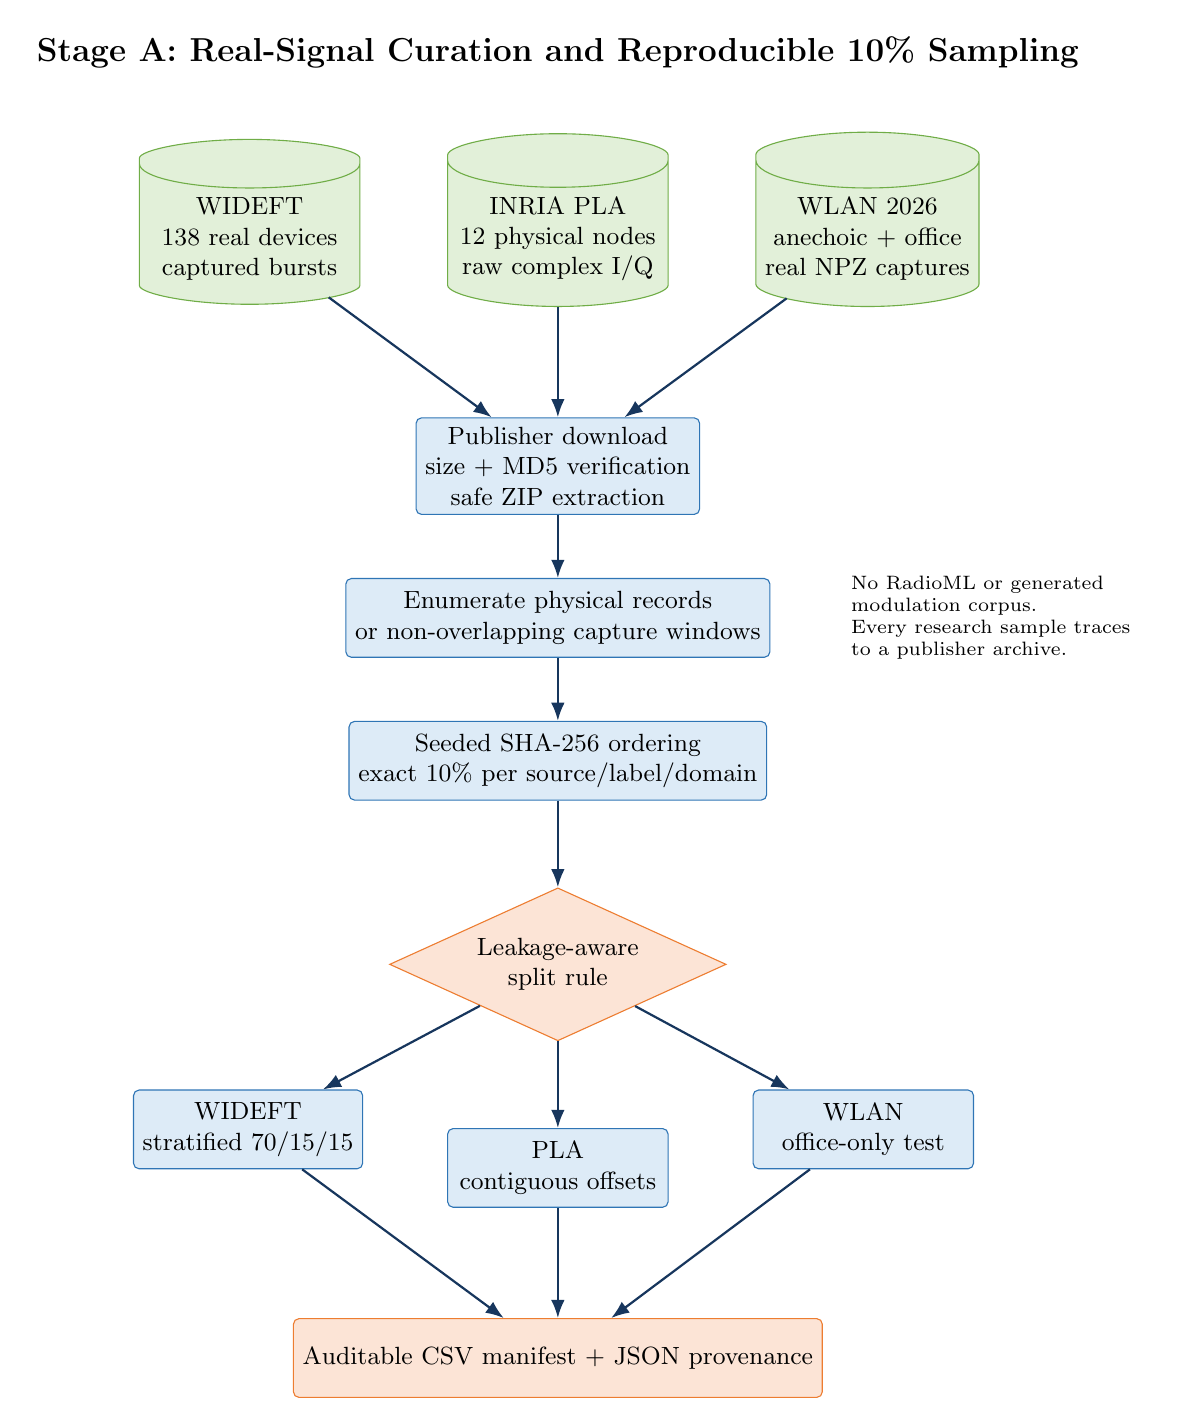
\begin{tikzpicture}[node distance=8mm and 11mm]
  \node[data] (wideft) {WIDEFT\\138 real devices\\captured bursts};
  \node[data, right=of wideft] (pla) {INRIA PLA\\12 physical nodes\\raw complex I/Q};
  \node[data, right=of pla] (wlan) {WLAN 2026\\anechoic + office\\real NPZ captures};

  \node[process, below=14mm of pla] (verify)
    {Publisher download\\size + MD5 verification\\safe ZIP extraction};
  \draw[arrow] (wideft) -- (verify);
  \draw[arrow] (pla) -- (verify);
  \draw[arrow] (wlan) -- (verify);

  \node[process, below=of verify] (enumerate)
    {Enumerate physical records\\or non-overlapping capture windows};
  \node[process, below=of enumerate] (subset)
    {Seeded SHA-256 ordering\\exact 10\% per source/label/domain};
  \node[decision, below=11mm of subset] (split) {Leakage-aware\\split rule};

  \node[process, below left=11mm and 14mm of split] (stratified)
    {WIDEFT\\stratified 70/15/15};
  \node[process, below=11mm of split] (contiguous)
    {PLA\\contiguous offsets};
  \node[process, below right=11mm and 14mm of split] (holdout)
    {WLAN\\office-only test};
  \node[output, below=14mm of contiguous] (manifest)
    {Auditable CSV manifest + JSON provenance};

  \draw[arrow] (verify) -- (enumerate);
  \draw[arrow] (enumerate) -- (subset);
  \draw[arrow] (subset) -- (split);
  \draw[arrow] (split) -- (stratified);
  \draw[arrow] (split) -- (contiguous);
  \draw[arrow] (split) -- (holdout);
  \draw[arrow] (stratified) -- (manifest);
  \draw[arrow] (contiguous) -- (manifest);
  \draw[arrow] (holdout) -- (manifest);

  \node[note, right=9mm of enumerate] {
    No RadioML or generated modulation corpus.\\
    Every research sample traces to a publisher archive.
  };

  \node[font=\bfseries\large, above=7mm of pla]
    {Stage A: Real-Signal Curation and Reproducible 10\% Sampling};
\end{tikzpicture}

% Page 2: model
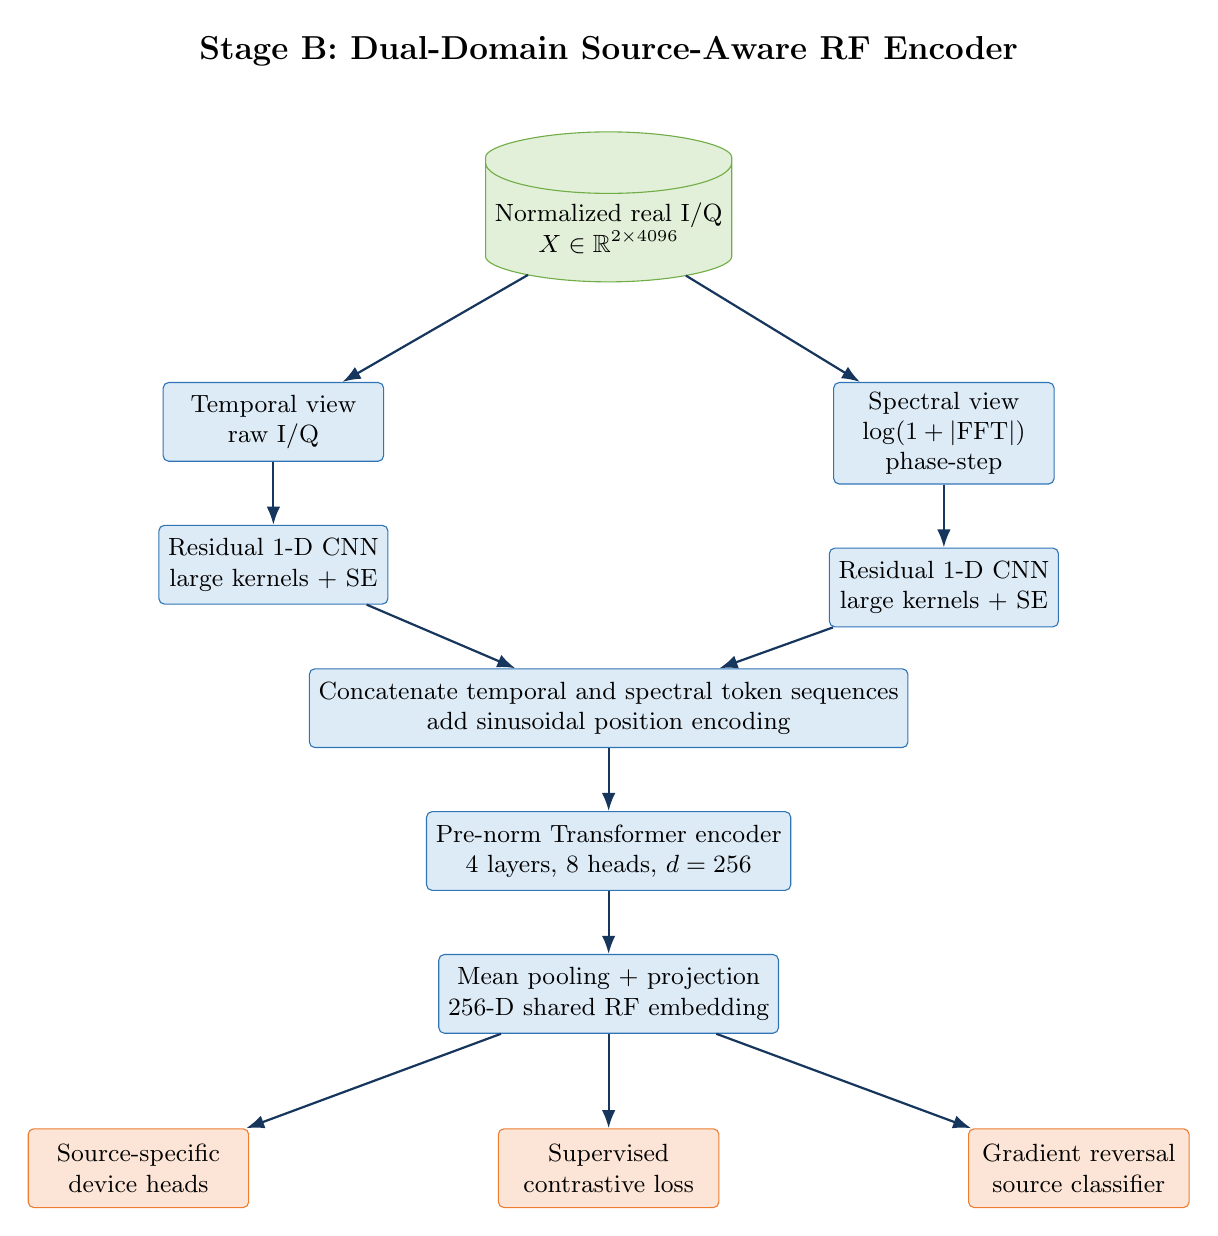
\begin{tikzpicture}[node distance=8mm and 11mm]
  \node[data] (input) {Normalized real I/Q\\$X\in\mathbb{R}^{2\times4096}$};

  \node[process, below left=13mm and 22mm of input] (timeview)
    {Temporal view\\raw I/Q};
  \node[process, below right=13mm and 22mm of input] (freqview)
    {Spectral view\\$\log(1+|\mathrm{FFT}|)$\\phase-step};

  \node[process, below=of timeview] (timecnn)
    {Residual 1-D CNN\\large kernels + SE};
  \node[process, below=of freqview] (freqcnn)
    {Residual 1-D CNN\\large kernels + SE};

  \node[process, below=18mm of input, yshift=-31mm] (tokens)
    {Concatenate temporal and spectral token sequences\\add sinusoidal position encoding};
  \node[process, below=of tokens] (transformer)
    {Pre-norm Transformer encoder\\4 layers, 8 heads, $d=256$};
  \node[process, below=of transformer] (embedding)
    {Mean pooling + projection\\256-D shared RF embedding};

  \node[output, below left=12mm and 24mm of embedding] (heads)
    {Source-specific\\device heads};
  \node[output, below=12mm of embedding] (supcon)
    {Supervised\\contrastive loss};
  \node[output, below right=12mm and 24mm of embedding] (domain)
    {Gradient reversal\\source classifier};

  \draw[arrow] (input) -- (timeview);
  \draw[arrow] (input) -- (freqview);
  \draw[arrow] (timeview) -- (timecnn);
  \draw[arrow] (freqview) -- (freqcnn);
  \draw[arrow] (timecnn) -- (tokens);
  \draw[arrow] (freqcnn) -- (tokens);
  \draw[arrow] (tokens) -- (transformer);
  \draw[arrow] (transformer) -- (embedding);
  \draw[arrow] (embedding) -- (heads);
  \draw[arrow] (embedding) -- (supcon);
  \draw[arrow] (embedding) -- (domain);

  \node[font=\bfseries\large, above=7mm of input]
    {Stage B: Dual-Domain Source-Aware RF Encoder};
\end{tikzpicture}

% Page 3: optimization
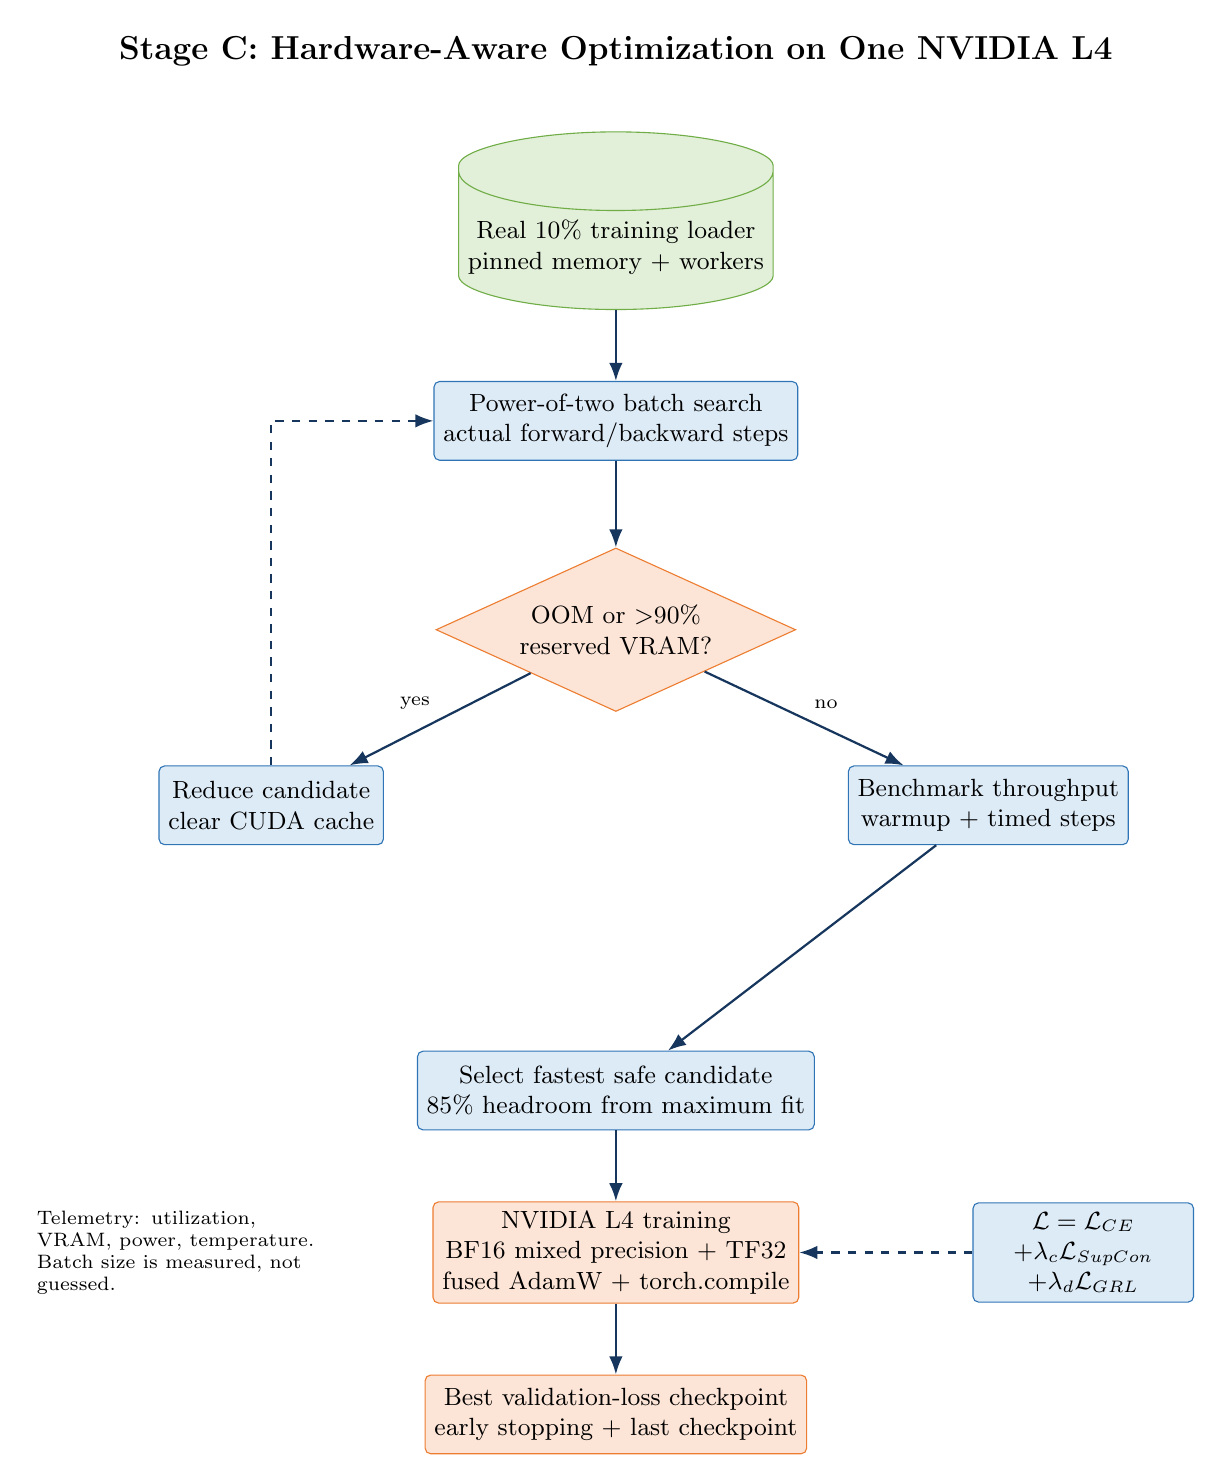
\begin{tikzpicture}[node distance=9mm and 12mm]
  \node[data] (batches) {Real 10\% training loader\\pinned memory + workers};
  \node[process, below=of batches] (search)
    {Power-of-two batch search\\actual forward/backward steps};
  \node[decision, below=11mm of search] (oom) {OOM or $>$90\%\\reserved VRAM?};
  \node[process, below left=12mm and 18mm of oom] (reduce)
    {Reduce candidate\\clear CUDA cache};
  \node[process, below right=12mm and 18mm of oom] (bench)
    {Benchmark throughput\\warmup + timed steps};
  \node[process, below=20mm of oom, yshift=-23mm] (select)
    {Select fastest safe candidate\\85\% headroom from maximum fit};
  \node[output, below=of select] (l4)
    {NVIDIA L4 training\\BF16 mixed precision + TF32\\fused AdamW + torch.compile};

  \node[process, right=22mm of l4] (loss)
    {$\mathcal{L}=\mathcal{L}_{CE}$\\
     $+\lambda_c\mathcal{L}_{SupCon}$\\
     $+\lambda_d\mathcal{L}_{GRL}$};
  \node[output, below=of l4] (checkpoint)
    {Best validation-loss checkpoint\\early stopping + last checkpoint};

  \draw[arrow] (batches) -- (search);
  \draw[arrow] (search) -- (oom);
  \draw[arrow] (oom) -- node[above left,font=\scriptsize]{yes} (reduce);
  \draw[arrow] (oom) -- node[above right,font=\scriptsize]{no} (bench);
  \draw[dashedarrow] (reduce) |- (search);
  \draw[arrow] (bench) -- (select);
  \draw[arrow] (select) -- (l4);
  \draw[arrow] (l4) -- (checkpoint);
  \draw[dashedarrow] (loss) -- (l4);

  \node[note, left=11mm of l4] {
    Telemetry: utilization, VRAM, power, temperature.\\
    Batch size is measured, not guessed.
  };
  \node[font=\bfseries\large, above=7mm of batches]
    {Stage C: Hardware-Aware Optimization on One NVIDIA L4};
\end{tikzpicture}

% Page 4: evaluation
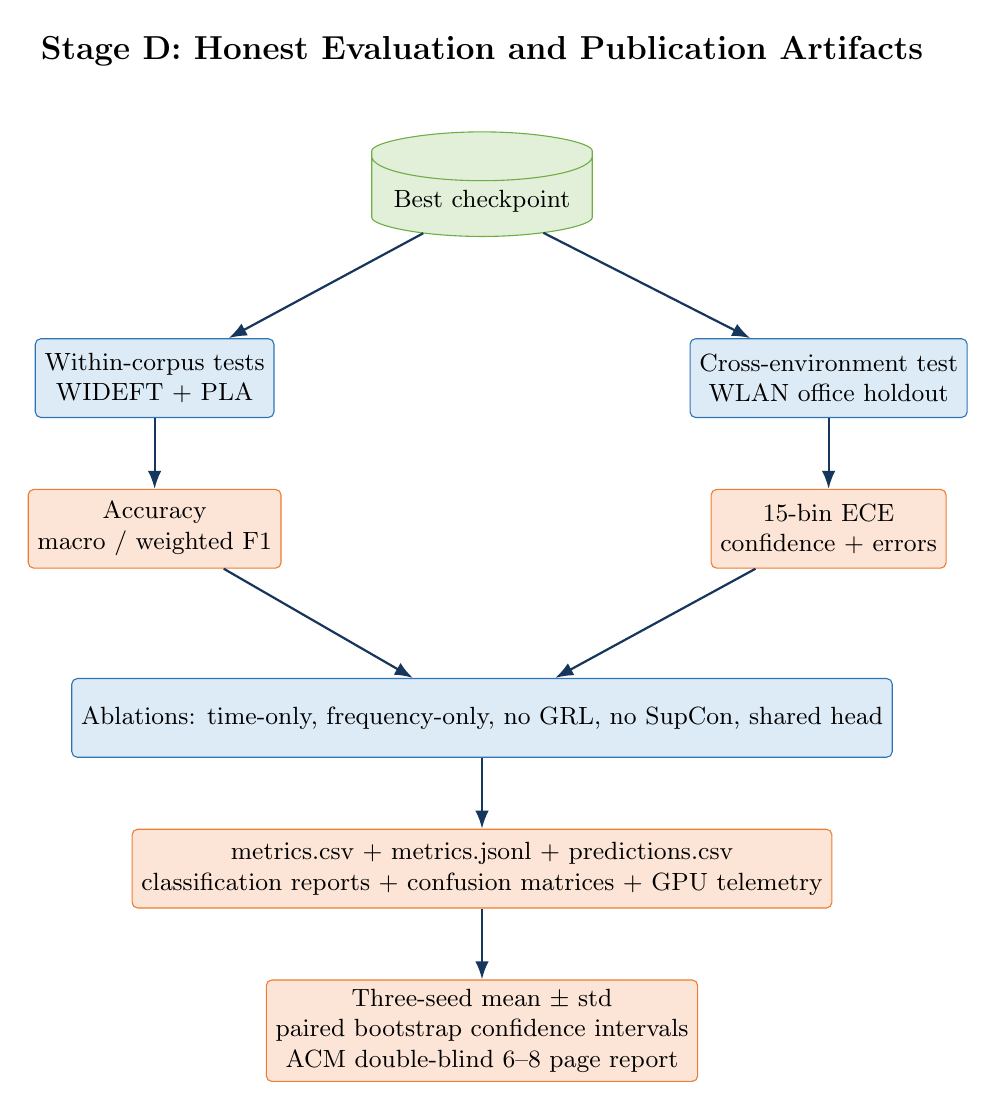
\begin{tikzpicture}[node distance=9mm and 12mm]
  \node[data] (checkpoint) {Best checkpoint};
  \node[process, below left=13mm and 22mm of checkpoint] (within)
    {Within-corpus tests\\WIDEFT + PLA};
  \node[process, below right=13mm and 22mm of checkpoint] (cross)
    {Cross-environment test\\WLAN office holdout};

  \node[output, below=of within] (metrics1)
    {Accuracy\\macro / weighted F1};
  \node[output, below=of cross] (metrics2)
    {15-bin ECE\\confidence + errors};

  \node[process, below=22mm of checkpoint, yshift=-34mm] (ablation)
    {Ablations: time-only, frequency-only, no GRL, no SupCon, shared head};
  \node[output, below=of ablation] (exports)
    {metrics.csv + metrics.jsonl + predictions.csv\\
     classification reports + confusion matrices + GPU telemetry};
  \node[output, below=of exports] (paper)
    {Three-seed mean $\pm$ std\\paired bootstrap confidence intervals\\
     ACM double-blind 6--8 page report};

  \draw[arrow] (checkpoint) -- (within);
  \draw[arrow] (checkpoint) -- (cross);
  \draw[arrow] (within) -- (metrics1);
  \draw[arrow] (cross) -- (metrics2);
  \draw[arrow] (metrics1) -- (ablation);
  \draw[arrow] (metrics2) -- (ablation);
  \draw[arrow] (ablation) -- (exports);
  \draw[arrow] (exports) -- (paper);

  \node[font=\bfseries\large, above=7mm of checkpoint]
    {Stage D: Honest Evaluation and Publication Artifacts};
\end{tikzpicture}

\end{document}
